% \IUref{IUAdmPS}{Administrar Planta de Selección}
% \IUref{IUModPS}{Modificar Planta de Selección}
% \IUref{IUEliPS}{Eliminar Planta de Selección}


% Copie este bloque por cada caso de uso:
%-------------------------------------- COMIENZA descripción del caso de uso.
\begin{figure}[htbp!]
		\centering
			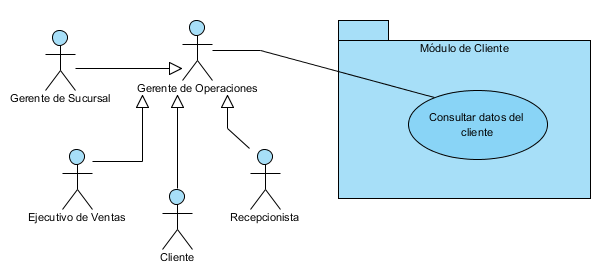
\includegraphics[width=0.8\textwidth]{images/ConsultarCliente}
		\caption{Diagrama de Casos de Uso del sistema.}
	\end{figure}

%\begin{UseCase}[archivo de imágen]{UCX}{Nombre del Caso de uso}{
	\begin{UseCase}{CU2}{Consultar datos del cliente.}{
		Permite consultar la información de los clientes para conocer las membresías, servicios y cursos que tiene relacionados.
	}
		\UCitem{Versión}{1.0}
		\UCitem{Actor}{Gerente de Operaciones, Gerente de Sucursal, Ejecutivo de Ventas, Recepcionista y Cliente.}
		\UCitem{Propósito}{Conocer la información personal, de contacto, ubicación y médica de los clientes, así como también, conocer las membresías, servicios y cursos que cada uno tiene.}
		\UCitem{Entradas}{Nombre del cliente o Clave CURP.}
		\UCitem{Origen}{Teclado.}
		\UCitem{Salidas}{Registro del cliente con información breve sobre él.}
		\UCitem{Destino}{Pantalla.}
		\UCitem{Precondiciones}{EL cliente debe contar con un registro previo.}
		\UCitem{Postcondiciones}{Ninguna.}
		\UCitem{Errores}{{\bf E6:} ``La clave CURP o nombre no existen'' -- El sistema muestra el Mensaje {\bf MSG7-}``La clave CURP o nombre no existen.'' y continua al paso 1.}		
		\UCitem{Tipo}{Caso de uso primario}
		\UCitem{Observaciones}{}
		\UCitem{Autor}{Roberto Mendoza Saavedra}
		\UCitem{Revisor}{}
	\end{UseCase}

	\begin{UCtrayectoria}{Principal}
		\UCpaso[\UCactor] Solicita la consulta de los datos de un cliente seleccionando la opción de ``Consultar clientes'' de la \IUref{IU4}{Pantalla principal empleados} o de la \IUref{IU5}{Pantalla de perfil} .
		\UCpaso Solicita el nombre del cliente o la clave CURP del cliente de la \IUref{IU5}{Pantalla de Consulta}.
		\UCpaso[\UCactor] Proporciona el nombre o la CURP.
		\UCpaso Verifica si la clave CURP o el nombre del cliente coincide con algún registro [E6].
		\UCpaso Muestra el registro del cliente con una información breve del mismo en la \IUref{IU5}{Pantalla de Consulta}.
		\UCpaso[\UCactor] Da clic sobre el registro del cliente y se muestra la pantalla \IUref{IU7}{Pantalla de Mostrar InfoCliente}.
		\UCpaso Arroja la información detallada del cliente de acuerdo a todos los datos otorgados al momento del registro del cliente.
		
	\end{UCtrayectoria}
	

		

	